\documentclass[10pt, oneside]{article}   	
\usepackage[margin=0.8in]{geometry}  
\usepackage[dvips]{graphics}
\usepackage{epsfig}
\usepackage{amsmath}
\usepackage{xspace}
\usepackage{fancybox}
\usepackage{graphicx,xspace,cite,verbatim,comment}
\usepackage[demo]{graphicx}
\usepackage{caption}
\usepackage{subcaption}
\usepackage{hyperref,array,color,balance,multirow}
\usepackage{balance,float,url,amsfonts,alltt}
\usepackage{mathtools,rotating,amsmath,amssymb}
\usepackage{color,cite,ifpdf,fancyvrb,array,listings}
\usepackage{algorithm,algpseudocode}
\usepackage{tabularx}
\usepackage{natbib}              		
\geometry{letterpaper}                   		
\usepackage{graphicx}		
\usepackage{subcaption}		
\usepackage{amssymb}

%SetFonts

%SetFonts


\title{\textbf{Best Matcher Explanation}}
\author{Zhiwei Fan\hspace{7ex}
	   Lingfeng Huang\hspace{7ex}
	   Fang Wang\\
	   zfan29@wisc.edu\hspace{3ex}
	   lhuang58@wisc.edu\hspace{3ex}
	   fwang64@wisc.edu
	   }
%\date{}							% Activate to display a given date or no date

\begin{document}
\maketitle 

\section*{Description of Data Generation and Transformation}
During the project stage 2, we have got around 70000 tuple pairs and observed that it was nearly impossible to get at least 50 positive
sample points (tuple pairs that match) from the 400 sampled tuple pairs during the labeling stage, thus we have performed \textit{reblocking}
adding additional blockers and blocking rules. 
\subsubsection*{Blockers Used in Re-blocking}
\textbf{Numeric Value Blocker:} \\
Calculating the \textit{absolute value} of \textit{difference} between {publishedYear, publishedMonth, publishedDay, pages} as \textit{yearDiff, monthDiff, dayDiff, pageDiff}. Any tuple pair
that is found to satisfy \textbf{\textit{any}} rules defined in \\ \{yearDiff$\leq$2, monthDiff$\leq$2, dayDiff$\leq$2, pageDiff$\leq$10\} will be filtered out.
\vspace{1ex}
\\
\textbf{Isbn Partial Blocker:}\\
Filtering out those tuple pairs got from the \textit{numeric\_value\_blocker} that \textit{do NOT} agree on the \textit{first four digits of isbn}
\vspace{1ex}
\\
\textbf{Title Rule-based Blocker:}\\
Filtering out those tuple pairs got from the previous two blockers described the jaccard similarity score of titles \textit{smaller} than 0.5.
\vspace{1ex}
\\
After conducting \textit{reblocking}, we have finally got 5369 tuple pairs in our \textit{new} \textit{tableC.csv}

\section*{Labeling}
After labeling and \textit{throw away}  those tuple pairs that we are not sure whether they match, we have finally got \textit{350} tuple pairs with 
\textit{\textbf{130 positive}} examples and \textit{\textbf{220 negative}} examples in our \textit{golden data} (tableH.csv). 

\section*{Feature Construction}
We have taken advantage of different \textit{similarity measurement} functions in \textit{py\_entitymatching} (e.g., py\_entitymatching.affine(s1,s2))
to construct both \textit{sequence-based} (e.g., py\_entitymatching.lev\_dist(s1, s2),) and \textit{set-based} (e.g., py\_entitymatching.jaccard(arr1, arr2))
features on the original \textit{string} attributes (title, author, publisher). We have also constructed features on original \textit{numeric} features 
(publishedYear, publishedMonth) using py\_entitymatching.rel\_diff(d1, d2) and py\_entitymatching.abs\_norm(d1, d2). \textit{publishedDay} is not
used due to its \textit{high variance} even in \textit{matching tuple pairs}. In total, we have constructed 42 features initially before performing any
feature selection.

\newpage

\section*{Development and Evaluation Sets}
After Randomly split the set H (gold data) into a development set I of 250 examples and an evaluation set J of 100 examples, we got the I and J
with the following statistical data:

\begin{table}[H]
\begin{tabular}{c}
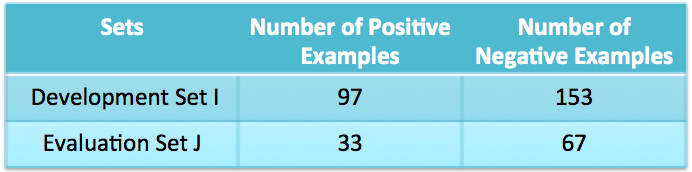
\includegraphics[width=4in]{sets}
\end{tabular}
\end{table}

\section*{Initial Cross Validation Measurement}
We have chosen several learning models and performed 10-fold cross validation on these models using the development dataset I. The corresponding \textit{\textbf{initial}}
(the first time) precision, recall and F-1 are shown as the following:

\begin{table}[H]
\begin{tabular}{c}
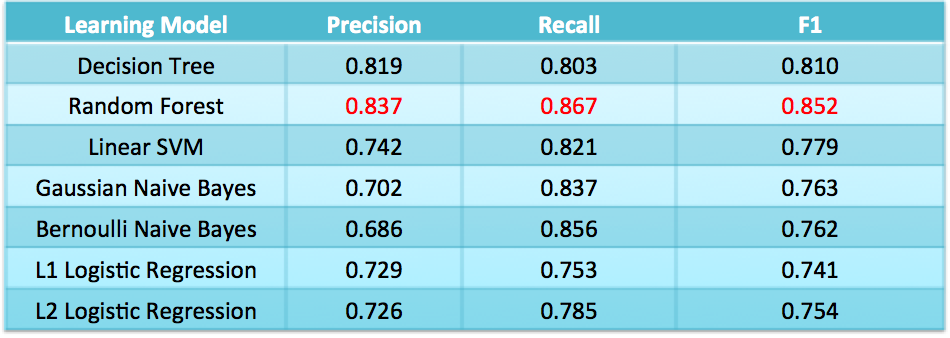
\includegraphics[width=4in]{initial_score}
\end{tabular}
\end{table}

\noindent
We have noticed that \textbf{\textit{random forest}} gave the best performance considering \textit{precision, recall}  and \textit{F1} together. However,  the fact
that F-1 score of \textit{random forest} is only 0.852 is not very promising. Thus, we continued to \textit{tune} the models and performed \textit{feature selection}
with the hope to improve F-1 score (as well as precision and recall) of \textit{random forest}.
 
\section*{Debugging Iterations}
We have first tuned \textit{random forest} itself. The parameters we have tuned include \textit{the number of trees, the maximal depth, the minimal sample split, the minimal samples leaf} and \textit{the maximal features to consider}.
Later on, we have performed \textit{feature selection} with \textit{backward selection} (each time reduce one feature and keeps the \textit{subset} of features that the maximal \textit{F-1 score} was observed). Two features 
\textit{author\_affine\_score} and \textit{publisher\_smith\_waterman\_score} and have achieved 0.923 \textit{precision}, 0.913 \textit{recall} and 0.918 \textit{F-1 score} in the \textit{10-fold cross validation} process on \textit{development set I}. Amazingly, on \textit{evaluation set J}, we have seen 0.941 \textit{precision}, 0.967 \textit{recall} and 0.954 \textit{F-1 score}. In order to get \textit{stable} result during the \textit{feature selection}, \textit{10 iterations} of experiments have been conducted, hundreds of experimental data has been used. For space saving reason, we omit those tedious data report and do not think these \textit{intermediate data} is necessary to be displayed.

\section*{Final Cross Validation Measurement and Measurement on Evaluation Set}
\subsection*{Final Cross Validation Measurement}
After tuning \textit{random forest} and performing \textit{feature selection}, we have re-run \textit{cross-validation} on development set I on all the models and the results are shown
as the following:
\begin{table}[H]
\begin{tabular}{c}
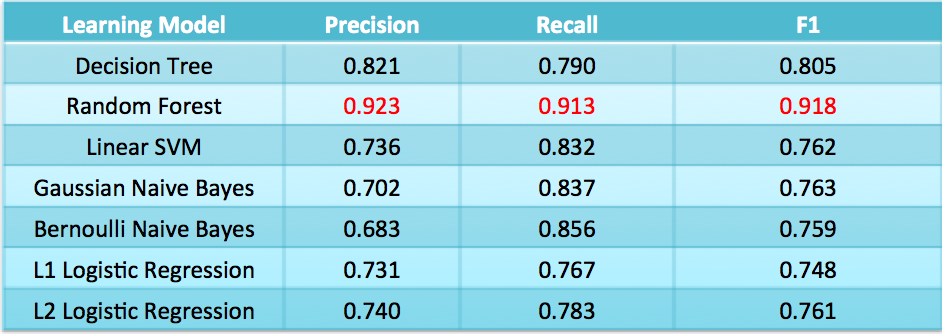
\includegraphics[width=4in]{final_cv_score}
\end{tabular}
\end{table}

\subsection*{Measurement on Evaluation Set}
Of course, we have \textit{evaluated} our \textit{final selected models random forest} along with \textit{other models}  on the \textit{evaluation set J} and the corresponding results are shown as the following:
\begin{table}[H]
\begin{tabular}{c}
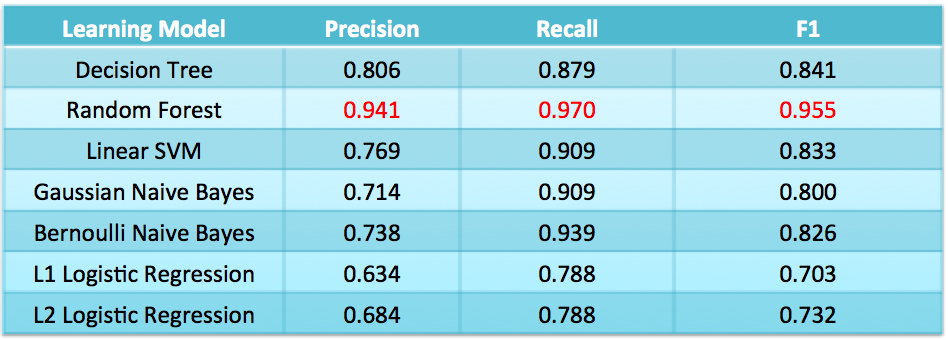
\includegraphics[width=4in]{final_eval_score}
\end{tabular}
\end{table}
 
\section*{List of final features in final feature set}
\{\_id, 
ltable\_id,
rtable\_id,
title\_affine\_score,
title\_lev\_dist\_score,
title\_lev\_sim\_score,
title\_jaro\_score,
title\_jaro\_winkler\_score,
title\_needleman\_wunsch\_score,
title\_smith\_waterman\_score,
title\_jaccard\_score,
title\_cosine\_score,
title\_overlap\_coeff\_score,
title\_dice\_score,
title\_monge\_elkan\_score, \\
author\_lev\_dist\_score,
author\_lev\_sim\_score,
author\_jaro\_score,
author\_jaro\_winkler\_score,
author\_needleman\_wunsch\_score,
author\_smith\_waterman\_score,
author\_jaccard\_score,
author\_cosine\_score,
author\_overlap\_coeff\_score,
author\_dice\_score,
author\_monge\_elkan\_score,\\
publisher\_affine\_score,
publisher\_lev\_dist\_score,
publisher\_lev\_sim\_score,
publisher\_jaro\_score,
publisher\_jaro\_winkler\_score,
publisher\_needleman\_wunsch\_score,
publisher\_jaccard\_score,
publisher\_cosine\_score,
publisher\_overlap\_coeff\_score,
publisher\_dice\_score,
publisher\_monge\_elkan\_score,\\
year\_rel\_diff,
year\_abs\_norm,
month\_rel\_diff,
month\_abs\_norm,
pages\_rel\_diff, 
pages\_abs\_norm\}


\section*{Approximate Time Estimation}
It took us approximately 6 hours to finish \textit{reblocking} and \textit{labeling}. We have spent most time \textit{tuning} models and \textit{perfoming feature selection}. A big amount of experiments have conducted
for us to detect the problems and give ideas of \text{model tuning}. The experimental stage took us approximately 10 hours. In total, approximately 20 hours have been spent on the whole process.

\section*{Discussion}
Since we have chosen the domain \textit{book}, it is very hard to come to an agreement on \textit{the standard of matching}. Books of different versions should be regarded as \textit{non-match}. But during the \textit{labeling}
stage, we have observed other factors that could significantly influence the \textit{matcher learning} and essentially \textit{matching} in a \textit{negative} way. For example, the same book could be published by different publishers
during totally different time; the book that has multiple authors could have \textit{different author information} on different source websites: one website lists partial of the authors of the book while the other website lists the rest.
These \textit{inconsistency} has greatly impacted the \textit{learning} process and prevent us from improving the quality of matcher to higher standard (with higher precision, recall and F-1).

\end{document}  